\documentclass{article}
\usepackage{geometry}
\usepackage{graphicx}
\usepackage{subfigure}
\usepackage{bm}
\usepackage{amsmath}
\usepackage{enumerate}

\geometry{left=2.5cm,right=2.5cm,top=2.5cm,bottom=2.5cm}
	\author{Dongying Wang}
         \title{Dielectric function and Reflectivity}
        
\begin{document}
	\maketitle
	\section{Complex refractive index}
		The refraction of light occurs when light advances into optically different media. The refraction of light is determined from the refractive index $n$ and, classically, $n$ is defined by

		\begin{equation}
			n = c/s
		\end{equation}

		in which, $c$ is speed of light in vacuum and $s$ is the one in media.\\

		When there is no light absorption in media, the propagation number $K$ is 

		\begin{equation}
			K = \frac{2\pi n}{\lambda}
		\end{equation}

		where $\lambda$ is the wavelength in vacuum. The electric field becomes

		\begin{equation}
			E = E_{t0}exp[i(\omega t - Kx + \delta)] = E_{t0}exp[i(\omega t - \frac{2\pi n}{\lambda}x + \delta)]
		\end{equation}

		where $E_{t0}$ corresponds to $E_{0}$ in the transparent medium and $\delta$ is a phase difference when the light crosses the interface. So the quantity $n$ represents how much wavelength changes in media. If there are media that show strong light absorption, and such a phenomenon cannot be expressed only with $n$. We introduce a complex refractive index $N$.

		\begin{equation}
			N = n - ik
		\end{equation}

		The electric field becomes

		\begin{equation}
			E = E_{t0}exp[i(\omega t - \frac{2\pi N}{\lambda}x + \delta)] = E_{t0}exp(-\frac{2\pi k}{\lambda})exp[i(\omega t - \frac{2\pi n}{\lambda}x + \delta)]
		\end{equation}

		Obviously, $exp(2\pi k/\lambda)$ represents absorption. (In oscillator model, the damping may be caused by interaction between next oscillators.) Comes to energy(square). There is an absorption coefficient $\alpha = 4\pi k/\lambda$

		\begin{figure} 
			\centering 
			\subfigure[No absorption]{ \label{fig:subfig:a} %% label for first subfigure 
			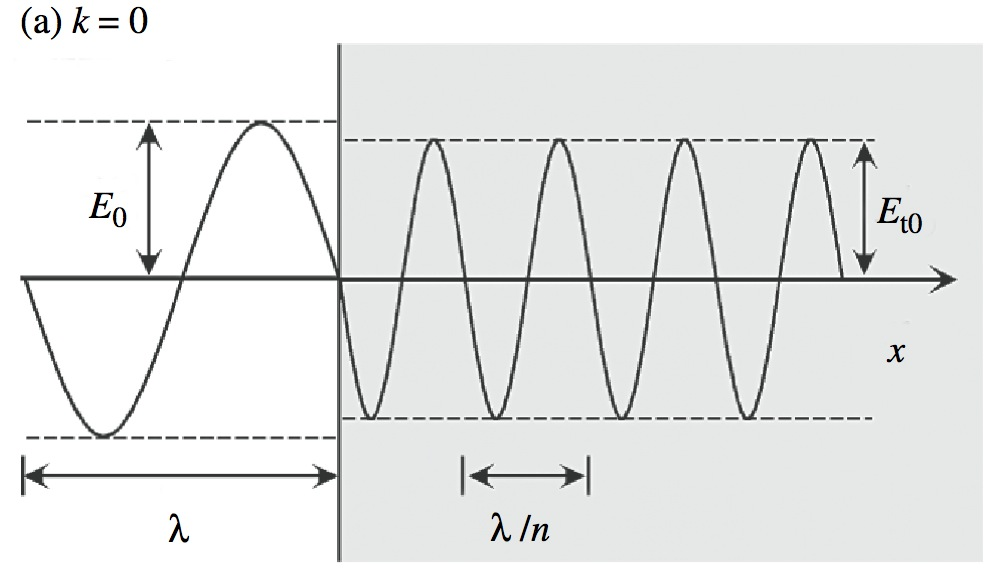
\includegraphics[height=1.7in]{fig1.jpg}} 
			%\hspace{1in} 
			\subfigure[Absorption]{ \label{fig:subfig:b} %% label for second subfigure 
			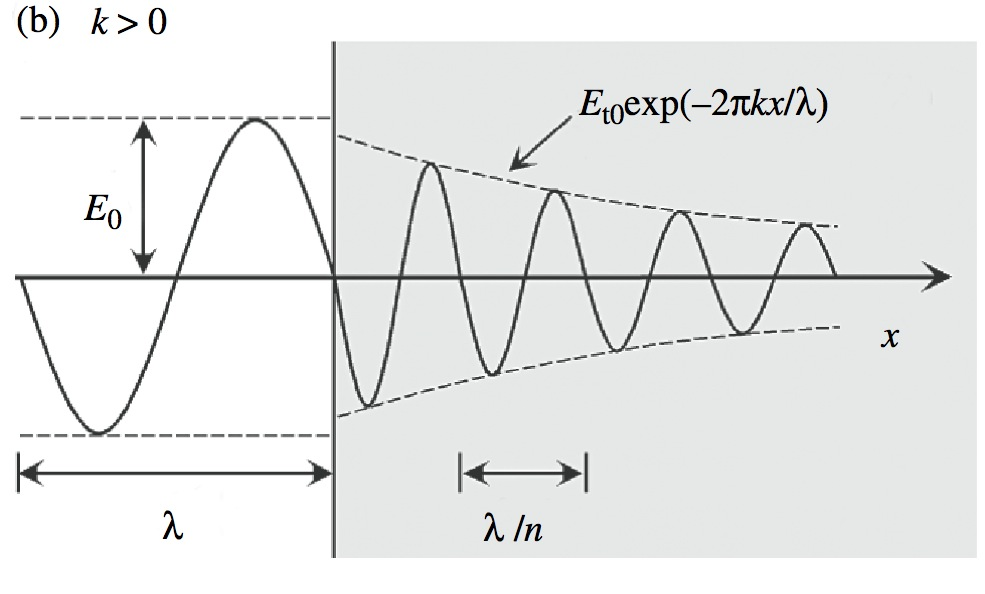
\includegraphics[height=1.7in]{fig2.jpg}} 
	
			\caption{Electric field in media} \label{fig:subfig} %% label for entire figure 
		\end{figure}

		\paragraph{Refractive index and Band gap}

			The imaginary part of the index describes wave decay. We can calculate stimulated absorption results in a wave to decay in a medium (optical loss).\\

			To begin with, we introduce the density of state $\rho(E)$, which means the number of states between $E$ and $E + dE$ over $VdE$. In the k-space each electronic state occupies a volume of $\frac{4\pi^{3}}{V}$, where $V$ is the volume of the system.

			\begin{equation}
			\begin{aligned}
				E_{c}(k_{c}) = E_{c} + \frac{\hbar k_{c}^{2}}{2m_{e}}\\
				E_{v}(k_{v}) = E_{v} + \frac{\hbar k_{v}^{2}}{2m_{h}}\\
				\hbar\omega \sim E_{c}(k_{e}) - E_{v}(k_{e}) = E_{gap} + \frac{\hbar k_{e}^{2}}{m_{e}}
			\end{aligned}
			\end{equation}

			where $c$ means conductor band, $v$ means valenced band $e$ means electrons, $h$ means holes.

			\begin{equation}
				\rho(E) = \rho(k)\cdot\frac{dk}{VdE} = \frac{4\pi k^{2}}{4\pi^{3}/V}\frac{dk}{VdE} = \frac{m_{e}}{2\pi^{2}\hbar^{3}}\sqrt{m_{e}(E - E_{c})}
			\end{equation}

			When the incident photon has an energy $E = \hbar\omega$,

			\begin{equation}
				\rho(\hbar\omega) = \frac{m_{e}}{2\pi^{2}\hbar^{3}}\sqrt{m_{e}(\hbar\omega - E_{gap})}
			\end{equation}

			Make a quantum correction(electrons are Fermions), the absorption coefficient $\alpha(\omega)$
			
			\begin{equation}
				\alpha(\omega)\hbar\omega = \rho(\hbar\omega)f_{c}(E_{c})(1 - f_{v}E_{v})
			\end{equation}

			As we already know $\alpha = 4\pi k/\lambda$, $k$ can be calculated now.


	\section{Dielectric constant}

		According to the Maxwell equation, the speed of light in vacuum can be expressed as

		\begin{equation}
			c = \sqrt{\mu_{0}\epsilon_{0}}
		\end{equation}

		And the one in media is

		\begin{equation}
			s = \sqrt{\mu\epsilon}
		\end{equation}

		For a material that is not magnetic the permeability is $\mu_{0}$, so that, according to the definition of refractive index

		\begin{equation}
			N = \frac{c}{s} = \sqrt{\epsilon/\epsilon_{0}} = \sqrt{\epsilon_{p}}
		\end{equation}

		\paragraph{Negative dielectric constant}
			A simple model for the dynamics of the displacement x of the bound electron is as follows

			\begin{equation}
				m\ddot{x} = eE - kx - m\gamma\dot{x}
			\end{equation}

			spring-like restoring force to the binding of the electron to nucleus, $\omega_{0}$ represents bounds between electrons.\\
			friction-type force proportional to the velocity of the electron, the frictional term $\gamma$ arises from collisions that tend to slow down the
			electron.

			\begin{equation}
			\begin{aligned}
				\epsilon(\omega) = \epsilon_{1}(\omega) - i\epsilon_{2}(\omega)\\
				\epsilon_{1} = \epsilon_{0} + \frac{\epsilon_{0}\omega_{p}^{2}(\omega_{0}^{2} - \omega^{2})}{(\omega_{0}^{2} - \omega^{2})^{2} + \gamma^{2}\omega^{2}} \ \ \ \ \ \ \ \ \ \epsilon_{2} = \frac{\epsilon_{0}\omega_{p}^{2}\omega\gamma}{(\omega_{0}^{2} - \omega^{2})^{2} + \gamma^{2}\omega^{2}}
			\end{aligned}
			\end{equation}

			This is Lorentz model. There are different conditions with three kinds of materials.

			\begin{itemize}
				\item Dielectrics, $\omega_{0} \neq 0,\ \ \gamma \neq 0.$
				\item Conductors, $\omega_{0} = 0,\ \ \gamma \neq 0.$
				\item Plasmas, $\omega_{0} = 0,\ \ \gamma = 0.$
			\end{itemize}

			For dielectrics, around the resonant frequency $\omega_{0}$, the real part $\epsilon_{1}$ behaves in an anomalous manner, that is, it drops rapidly with frequency to values less than $\epsilon_{0}$ and the material exhibits strong absorption.\\

			For conductors and plasmas, when $\omega$ is low enough, the real part $\epsilon_{1}$ can be negative.



\end{document}